\chapter{Fase B: Arsitektur Bisnis}

\section{Tujuan}
Tujuan utama dari Pengembangan Arsitektur Bisnis adalah sebagai berikut:
\begin{enumerate}
	\item Membangun Arsitektur Bisnis Target yang menjelaskan bagaimana perusahaan seharusnya beroperasi untuk mencapai tujuan bisnis, serta menanggapi pendorong strategis bisnis (\textit{business strategic drivers}) yang telah ditetapkan dalam Visi Arsitektur. Target arsitektur yang harus memenuhi atau menjawab \textit{Permintaan Pekerjaan Arsitektur} dan menjawab kekhawatiran para pemangku kepentingan (\textit{stakeholders}).
	\item Mengidentifikasi komponen dari Peta Jalan Arsitektur (\textit{architecture roadmap}) berdasarkan kesenjangan (\textit{gap}) antara Arsitektur Saat Ini dan Arsitektur Bisnis Target.
\end{enumerate}

\section{Input}
Input yang penting untuk Pengembangan Arsitektur Bisnis adalah sebagai berikut. Pada umumnya output dari fase-fase sebelumnya menjadi input pada fase ini. Pembahasan setiap item input pada fase ini bisa dilhat pada pembahasan mereka di fase-fase (bab-bab) sebelumnya.
\begin{enumerate}
	\item Prinsip bisnis, tujuan bisnis, dan pendorong bisnis
	\item Penilaian Kapabilitas
	\item Rencana Komunikasi
	\item Model Organisasi untuk Arsitektur Perusahaan
	\item Kerangka Arsitektur yang Disesuaikan
	\item Pernyataan Pekerjaan Arsitektur yang telah disetujui
	\item Prinsip Arsitektur, termasuk prinsip bisnis yang telah ada sebelumnya
	\item Company Continuum
	\item Repositori Arsitektur
	\item Visi Arsitektur, termasuk:
	\begin{itemize}
		\item Masalah
		\item Tujuan Pernyataan Pekerjaan Arsitektur
		\item Ringkasan gambaran umum
		\item Skenario bisnis (opsional)
		\item Persyaratan pemangku kepentingan tingkat tinggi secara rinci
	\end{itemize}
	\item Draf Dokumen Definisi Arsitektur, termasuk (jika dalam cakupan):
	\begin{itemize}
		\item Arsitektur Bisnis Dasar (tingkat tinggi)
		\item Arsitektur Data Dasar (tingkat tinggi)
		\item Arsitektur Aplikasi Dasar (tingkat tinggi)
		\item Arsitektur Teknologi Dasar (tingkat tinggi)
		\item Arsitektur Bisnis Target (tingkat tinggi)
		\item Arsitektur Data Target (tingkat tinggi)
		\item Arsitektur Aplikasi Target (tingkat tinggi)
		\item Arsitektur Teknologi Target (tingkat tinggi)
	\end{itemize}
	\item Permintaan untuk Pekerjaan Arsitektur
\end{enumerate}

\section{Langkah-Langkah}
Langkah-langkah dalam Pengembangan Arsitektur Bisnis adalah sebagai berikut:
\begin{enumerate}
	\item Memilih model referensi, sudut pandang dari berbagai aktor, dan alat
	\item Mengembangkan Deskripsi Arsitektur Bisnis Saat Ini
	\item Mengembangkan Deskripsi Arsitektur Bisnis Target
	\item Melakukan Analisis Kesenjangan
	\item Menentukan komponen dari peta jalan
	\item Membuat solusi untuk dampak atau efek samping di seluruh Lanskap Arsitektur
	\item Melakukan tinjauan formal pemangku kepentingan terhadap arsitektur yang diusulkan
	\item Menyelesaikan Arsitektur Bisnis
	\item Membuat Dokumen Definisi Arsitektur
\end{enumerate}

\subsection*{Contoh:}
Berikut adalah contoh penerapan langkah-langkah pengembangan arsitektur bisnis dalam konteks Hybrid Teaching and Learning di universitas:

\begin{enumerate}
	\item \textbf{Memilih model referensi, sudut pandang dari berbagai aktor, dan alat:}  
	Dalam konteks Hybrid Teaching and Learning, model referensi yang dipilih dapat berupa model pendidikan campuran (blended learning) yang menggabungkan pembelajaran daring dan luring. Sudut pandang yang dipertimbangkan termasuk dari sisi mahasiswa, dosen, staf IT, serta administrasi universitas. Alat yang dipilih mencakup platform LMS (Learning Management System) seperti Moodle, Zoom untuk pembelajaran daring, dan infrastruktur fisik kampus untuk pembelajaran luring.
	
	\item \textbf{Mengembangkan Deskripsi Arsitektur Bisnis Saat Ini:}  
	Deskripsi arsitektur saat ini mungkin mencakup penggunaan pembelajaran tatap muka secara dominan sebelum pandemi, dengan sistem pendukung minimal untuk pembelajaran daring. Infrastruktur teknologi yang ada mungkin terbatas pada penggunaan email dan forum diskusi.
	
	\item \textbf{Mengembangkan Deskripsi Arsitektur Bisnis Target:}  
	Arsitektur target dapat menggambarkan integrasi penuh antara pembelajaran daring dan luring, dengan platform digital yang kuat untuk manajemen konten, interaksi kelas, penilaian, dan pelaporan. Sistem harus mendukung fleksibilitas bagi mahasiswa untuk memilih mode belajar yang sesuai, baik dari rumah maupun kampus.
	
	\item \textbf{Melakukan Analisis Kesenjangan:}  
	Analisis kesenjangan dilakukan dengan membandingkan infrastruktur dan proses pembelajaran saat ini dengan target hybrid. Misalnya, kesenjangan dapat ditemukan pada kurangnya platform pembelajaran yang mudah diakses, kurangnya pelatihan bagi dosen untuk mengajar secara efektif secara daring, dan kebutuhan akan peningkatan infrastruktur jaringan di kampus.
	
	\item \textbf{Menentukan Komponen dari Peta Jalan:}  
	Komponen dari peta jalan untuk mengimplementasikan Hybrid Teaching and Learning mungkin mencakup pelatihan dosen tentang platform daring, peningkatan kapasitas server untuk mendukung akses mahasiswa, serta pengembangan kebijakan fleksibel mengenai kehadiran dan penilaian.
	
	\item \textbf{Membuat Solusi untuk Dampak atau Efek Samping di Seluruh Lanskap Arsitektur:}  
	Solusi untuk dampak potensial mungkin termasuk memastikan bahwa ada dukungan teknis yang memadai untuk mahasiswa dan dosen dalam menggunakan platform daring, mengatasi potensi kesenjangan akses teknologi di antara mahasiswa, dan memitigasi kekhawatiran mengenai interaksi sosial yang terbatas pada pembelajaran daring.
	
	\item \textbf{Melakukan Tinjauan Formal Pemangku Kepentingan terhadap Arsitektur yang Diusulkan:}  
	Tinjauan dilakukan oleh dekan, kepala departemen, dosen, mahasiswa, dan staf IT untuk memastikan bahwa solusi hybrid yang diusulkan memenuhi kebutuhan dan kemampuan seluruh pemangku kepentingan, baik dari segi teknologi, akademik, maupun administratif.
	
	\item \textbf{Menyelesaikan Arsitektur Bisnis:}  
	Setelah tinjauan pemangku kepentingan, rencana arsitektur final diselesaikan dengan penyesuaian sesuai umpan balik yang diberikan. Solusi hybrid final melibatkan sistem yang terintegrasi dengan baik antara pembelajaran daring dan luring, memastikan kemudahan transisi di antara keduanya.
	
	\item \textbf{Membuat Dokumen Definisi Arsitektur:}  
	Dokumen ini akan mencakup deskripsi detail tentang arsitektur hybrid yang diusulkan, termasuk platform teknologi yang digunakan, prosedur operasional, kebijakan pembelajaran, serta peta jalan implementasi secara menyeluruh.
\end{enumerate}

\section{Output}
Output yang diharapkan dari fase ini meliputi:
\begin{enumerate}
	\item Pernyataan Pekerjaan Arsitektur yang diperbarui sesuai kebutuhan
	\item Prinsip bisnis, tujuan bisnis, dan pendorong bisnis yang divalidasi
	\item Prinsip Arsitektur Bisnis yang diperbarui
	\item Draf Dokumen Definisi Arsitektur, termasuk konten yang diperbarui
	\item Draf Spesifikasi Persyaratan Arsitektur, termasuk konten yang diperbarui
	\item Komponen Arsitektur Bisnis dari Peta Jalan Arsitektur
\end{enumerate}

\subsection*{Contoh:}
Berikut adalah contoh penerapan elemen-elemen keluaran arsitektur bisnis dalam konteks Hybrid Teaching and Learning di universitas:

\begin{enumerate}
	\item \textbf{Pernyataan Pekerjaan Arsitektur yang diperbarui sesuai kebutuhan:}  
	Dalam konteks Hybrid Teaching and Learning, pernyataan pekerjaan arsitektur dapat diperbarui untuk mencerminkan perubahan dalam strategi pembelajaran yang melibatkan metode daring dan luring. Ini termasuk penambahan spesifikasi teknis untuk platform e-learning yang digunakan serta prosedur untuk dukungan teknologi dan pengembangan kurikulum berbasis hybrid.
	
	\item \textbf{Prinsip bisnis, tujuan bisnis, dan pendorong bisnis yang divalidasi:}  
	Prinsip-prinsip dan tujuan yang divalidasi untuk universitas dalam sistem hybrid dapat mencakup fleksibilitas dalam metode pengajaran, peningkatan aksesibilitas pembelajaran bagi mahasiswa dari berbagai lokasi, serta pengurangan hambatan fisik dalam proses pembelajaran. Pendorong bisnis mungkin meliputi efisiensi operasional dan peningkatan daya tarik bagi mahasiswa internasional.
	
	\item \textbf{Prinsip Arsitektur Bisnis yang diperbarui:}  
	Prinsip-prinsip arsitektur bisnis dapat diperbarui (ditambahkan, dihapus, dsb.) untuk memastikan bahwa teknologi digital dan infrastruktur fisik universitas mendukung metode pembelajaran hybrid. Contoh, misalnya penambahan prinsip-prinsip: fokus pada interoperabilitas platform teknologi, kelancaran transisi antara mode daring dan luring, serta kesesuaian dengan tujuan institusi.
	
	\item \textbf{Draf Dokumen Definisi Arsitektur, termasuk konten yang diperbarui:}  
	Dalam draf dokumen ini, arsitektur hybrid akan dijabarkan, mencakup komponen-komponen teknologi seperti Learning Management System (LMS), sistem komunikasi daring (misalnya Zoom atau Microsoft Teams), serta infrastruktur fisik kampus yang siap mendukung pembelajaran tatap muka dan daring secara bersamaan.
	
	\item \textbf{Draf Spesifikasi Persyaratan Arsitektur, termasuk konten yang diperbarui:}  
	Spesifikasi persyaratan arsitektur akan diperbarui untuk mencerminkan kebutuhan teknologi dan operasional yang lebih rinci, seperti persyaratan bandwidth internet, kebutuhan perangkat keras di ruang kelas, dan standar keamanan data yang digunakan dalam sistem pembelajaran daring.
	
	\item \textbf{Komponen Arsitektur Bisnis dari Peta Jalan Arsitektur:}  
	Komponen arsitektur bisnis untuk peta jalan akan mencakup pengembangan bertahap infrastruktur teknologi, pelatihan staf dan dosen untuk mengoperasikan sistem hybrid, serta penjadwalan transisi dari sistem pembelajaran tatap muka tradisional menuju metode hybrid yang lebih adaptif.
\end{enumerate}

\section{Menggunakan Repositori Arsitektur dan \textit{Enterprise Continuum}}
Tim arsitektur perlu mempertimbangkan sumber daya Arsitektur Bisnis yang relevan dari Repositori Arsitektur atau dari \textit{Enterprise Continuum} (solusi dan standar dari umum sampai spesifik), terutama:
\begin{enumerate}
	\item Standar umum yang berlaku (standard internasional dan nasional)
	\item Model bisnis umum yang relevan dengan sektor industri organisasi (industri pendidikan)
	\item Model bisnis yang relevan dengan domain bisnis (industri pendidikan tinggi)
	\item Blok bangunan spesifik perusahaan (spesifik terhadap universitas tersebut)
\end{enumerate}

\subsection{Contoh:}
Dalam penerapan Hybrid Teaching and Learning di universitas, tim arsitektur perlu mempertimbangkan sumber daya Arsitektur Bisnis yang relevan dari Repositori Arsitektur atau dari \textit{Enterprise Continuum}. Berikut adalah contoh penerapannya:

\begin{enumerate}
	\item \textbf{Standar umum yang berlaku:}  
	Standar internasional dan nasional yang relevan mencakup standar teknologi pembelajaran seperti ISO/IEC 40180 untuk sistem e-learning, dan standar aksesibilitas web (seperti WCAG 2.1) yang memastikan bahwa platform daring dapat diakses oleh semua mahasiswa, termasuk mereka yang memiliki keterbatasan fisik. Di tingkat nasional, pedoman dari Kementerian Pendidikan terkait pembelajaran digital juga harus dipatuhi.
	
	\item \textbf{Model bisnis umum yang relevan dengan sektor industri pendidikan:}  
	Model bisnis dalam sektor industri pendidikan mencakup penyediaan layanan pendidikan berkualitas yang dapat diakses secara daring dan luring, dengan fokus pada peningkatan pengalaman belajar mahasiswa melalui teknologi. Contoh penerapannya adalah integrasi LMS (Learning Management System) dengan sistem administrasi akademik yang memudahkan manajemen pembelajaran dan administrasi universitas.
	
	\item \textbf{Model bisnis yang relevan dengan domain bisnis pendidikan tinggi:}  
	Dalam konteks pendidikan tinggi, model bisnis hybrid teaching melibatkan penyusunan program kuliah yang fleksibel, penyediaan kuliah daring bagi mahasiswa yang tidak dapat hadir di kampus, dan integrasi evaluasi pembelajaran secara digital. Selain itu, kolaborasi antara dosen dan mahasiswa dapat diperluas dengan penggunaan platform digital untuk seminar atau kuliah tamu dari pakar luar negeri.
	
	\item \textbf{Blok bangunan spesifik universitas:}  
	Blok bangunan spesifik universitas meliputi infrastruktur teknologi seperti ruang kelas pintar yang dilengkapi perangkat audio-visual, jaringan internet berkecepatan tinggi, platform LMS khusus yang disesuaikan dengan kebutuhan universitas, serta kebijakan internal yang mengatur penggunaan teknologi dalam pembelajaran hybrid. Selain itu, termasuk pengembangan modul pelatihan bagi dosen untuk mengoptimalkan pembelajaran daring.
\end{enumerate}


\section{Identifikasi Katalog, Matriks, dan Diagram}
\begin{enumerate}
	\item Katalog mengumpulkan inventaris aset inti bisnis.
	\item Matriks menunjukkan hubungan antara entitas model.
	\item Diagram menggambarkan informasi Arsitektur Bisnis dari berbagai perspektif (sudut pandang).
\end{enumerate}

\subsection{Contoh:}
Dalam konteks Hybrid Teaching and Learning di universitas, identifikasi Katalog, Matriks, dan Diagram dapat diterapkan sebagai berikut:

\begin{enumerate}
	\item \textbf{Katalog:}  
	Katalog mengumpulkan inventaris aset inti yang digunakan dalam pembelajaran hybrid. Contoh aset inti di universitas meliputi:
	\begin{itemize}
		\item \textbf{Katalog Sumber Daya Digital:} Buku elektronik, jurnal akademik daring, video pembelajaran, dan modul interaktif yang tersedia dalam platform LMS.
		\item \textbf{Katalog Perangkat Keras:} Laptop, tablet, proyektor, dan peralatan audio-visual yang digunakan dalam pengajaran luring maupun daring.
		\item \textbf{Katalog Kursus:} Daftar semua kursus yang ditawarkan secara hybrid, termasuk deskripsi, jadwal, dan metodologi pengajaran.
		\item \textbf{Katalog Dosen:} Informasi mengenai dosen yang mengajar di program hybrid, termasuk kualifikasi, pengalaman, dan area keahlian.
		\item \textbf{Katalog Alat dan Aplikasi:} Daftar aplikasi dan alat yang digunakan dalam pembelajaran, seperti platform komunikasi (Zoom, Microsoft Teams), alat kolaborasi (Google Workspace), dan perangkat lunak pengelolaan kelas.
	\end{itemize}
	
	\item \textbf{Matriks:}  
	Matriks menunjukkan hubungan antara berbagai entitas dalam model pembelajaran hybrid. Contoh dalam konteks universitas adalah:
	\begin{itemize}
		\item \textbf{Matriks Keterkaitan Kursus dan Dosen:} Matriks ini menunjukkan hubungan antara dosen yang mengajar dan kursus yang ditawarkan. Misalnya, kolom mencantumkan nama dosen, sedangkan baris mencantumkan nama kursus. Sel-sel di dalam matriks dapat diisi dengan tanda centang atau nilai yang menunjukkan apakah seorang dosen mengajar kursus tertentu.
		
		\item \textbf{Matriks Keterlibatan Mahasiswa:} Matriks yang menunjukkan keterlibatan mahasiswa dalam pembelajaran daring versus luring. Kolom dapat mencakup nama mahasiswa, sedangkan baris mencakup aktivitas pembelajaran seperti mengikuti kuliah luring, menghadiri sesi diskusi daring, atau mengerjakan tugas daring. Sel-sel dapat diisi dengan nilai keterlibatan (misalnya, 0-100\%).
		
		\item \textbf{Matriks Kompetensi:} Matriks ini menunjukkan kompetensi yang diharapkan dari mahasiswa dalam setiap kursus. Baris dapat mencantumkan kompetensi yang diperlukan (misalnya, analisis data, keterampilan presentasi), sedangkan kolom mencantumkan kursus. Sel-sel di dalam matriks dapat diisi dengan tingkat penguasaan (misalnya, dasar, menengah, lanjutan).
		
		\item \textbf{Matriks Hubungan Alat Pembelajaran:} Matriks ini menunjukkan hubungan antara alat pembelajaran yang digunakan dan kursus yang ditawarkan. Baris mencantumkan alat pembelajaran (misalnya, Zoom, Google Classroom), sedangkan kolom mencantumkan kursus. Sel-sel dapat diisi dengan tanda centang yang menunjukkan alat mana yang digunakan dalam kursus tertentu.
	\end{itemize}
	
	\item \textbf{Diagram:}  
	Diagram digunakan untuk menggambarkan informasi Arsitektur Bisnis Hybrid Teaching and Learning dari berbagai perspektif. Contohnya, diagram dapat menunjukkan alur interaksi antara mahasiswa dan dosen dalam platform LMS, menggambarkan proses administrasi pengelolaan kelas hybrid, atau diagram alur kerja terkait pengelolaan materi ajar daring dan luring. Jenis-jenis diagram yang dapat digunakan antara lain:
	\begin{itemize}
		\item \textbf{Diagram Alur (Flowchart):} Untuk menggambarkan langkah-langkah dalam proses pengajaran dan pembelajaran.
		\item \textbf{Diagram Venn:} Untuk menunjukkan hubungan antara komponen pembelajaran daring dan luring.
		\item \textbf{Diagram Aktivitas:} Untuk memvisualisasikan aktivitas dan interaksi dalam pembelajaran hybrid.
		\item \textbf{Diagram Komponen:} Untuk menggambarkan komponen sistem yang terlibat dalam pembelajaran hybrid, termasuk perangkat lunak dan hardware.
		\item \textbf{Diagram Sekuen:} Untuk menunjukkan urutan interaksi antara mahasiswa, dosen, dan sistem LMS.
	\end{itemize}
\end{enumerate}


\section{Isi Dokumen Definisi Arsitektur}
\label{sec:isi_dokumen_definisi_arsitektur}
Isi utama dari Dokumen Definisi Arsitektur adalah sebagai berikut:
\begin{enumerate}
	\item Cakupan
	\item Tujuan, sasaran, dan kendala
	\item Prinsip arsitektur
	\item Arsitektur baseline dan target
	\item Model arsitektur (untuk setiap kondisi yang dimodelkan), seperti model untuk Arsitektur Bisnis, Arsitektur Data, Arsitektur Aplikasi, dan Arsitektur Teknologi
	\item Alasan dan justifikasi pendekatan arsitektural
	\item Pemetaan ke Repositori Arsitektur, termasuk pemetaan ke Lanskap Arsitektur, model referensi, standar, serta penilaian penggunaan kembali
	\item Analisis kesenjangan
	\item Penilaian dampak
	\item Arsitektur Transisional
\end{enumerate}

\subsection{Contoh:}
Dalam konteks Hybrid Teaching and Learning di universitas, isi dari Dokumen Definisi Arsitektur dapat diterapkan sebagai berikut:

\begin{enumerate}
	\item \textbf{Cakupan:}  
	Cakupan dokumen ini mencakup seluruh aspek Arsitektur Bisnis yang mendukung model pembelajaran hybrid, termasuk:
	\begin{itemize}
		\item Integrasi sistem pembelajaran daring dengan pembelajaran tatap muka.
		\item Proses pengelolaan kelas yang efektif baik untuk sesi online maupun offline.
		\item Penyediaan sumber daya belajar yang dapat diakses oleh mahasiswa di mana saja.
	\end{itemize}
	
	\item \textbf{Tujuan, sasaran, dan kendala:}  
	Tujuan dari arsitektur ini adalah untuk meningkatkan efektivitas pembelajaran dengan memanfaatkan teknologi, sementara sasaran mencakup:
	\begin{itemize}
		\item Mengurangi ketidakhadiran mahasiswa dalam perkuliahan.
		\item Meningkatkan interaksi antara mahasiswa dan dosen.
	\end{itemize}
	Kendala yang mungkin dihadapi termasuk:
	\begin{itemize}
		\item Keterbatasan teknologi (misalnya, koneksi internet yang tidak stabil).
		\item Resistensi terhadap perubahan dari dosen dan mahasiswa.
	\end{itemize}
	
	\item \textbf{Prinsip arsitektur:}  
	Prinsip yang mendasari arsitektur ini mencakup:
	\begin{itemize}
		\item Fleksibilitas dalam metode pengajaran (misalnya, pilihan antara kuliah daring atau tatap muka).
		\item Aksesibilitas sumber daya pendidikan (misalnya, materi kuliah yang dapat diunduh).
	\end{itemize}
	
	\item \textbf{Arsitektur \textit{baseline} dan target:}  
	Arsitektur baseline dan target (lihat Subbab \ref{sec:isi_komponen_arsitektur_bisnis}).
	
	
	\item \textbf{Model arsitektur:}  
	Berbagai model arsitektur yang dapat dikembangkan antara lain:
	\begin{itemize}
		\item \textbf{Model Arsitektur Bisnis:} Menggambarkan struktur organisasi dan proses bisnis, seperti pengelolaan kelas campuran.
		\item \textbf{Model Arsitektur Data:} Menjelaskan bagaimana data akademik (nilai, absensi) dikelola dalam sistem pembelajaran.
		\item \textbf{Model Arsitektur Aplikasi:} Mencakup aplikasi seperti Zoom untuk perkuliahan daring dan Google Drive untuk berbagi materi.
		\item \textbf{Model Arsitektur Teknologi:} Menggambarkan infrastruktur yang mendukung, seperti jaringan Wi-Fi di kampus dan perangkat keras yang digunakan oleh mahasiswa.
	\end{itemize}
	
	\item \textbf{Alasan dan justifikasi pendekatan arsitektural:}  
	Pendekatan ini dijustifikasi dengan mengacu pada:
	\begin{itemize}
		\item Kebutuhan untuk mengadaptasi metode pengajaran yang efektif di era digital.
		\item Meningkatnya permintaan untuk pembelajaran yang fleksibel dan aksesibel dari mahasiswa.
	\end{itemize}
	
	\item \textbf{Pemetaan ke Repositori Arsitektur:}  
	Dokumen ini harus memetakan elemen-elemen arsitektur ke dalam repositori arsitektur yang ada, termasuk:
	\begin{itemize}
		\item Hubungan antara model referensi, seperti TOGAF, dengan implementasi di universitas.
		\item Penilaian penggunaan kembali sumber daya pendidikan yang ada, seperti materi kuliah yang sudah tersedia secara daring.
	\end{itemize}
	
	\item \textbf{Analisis kesenjangan:}  
	Melakukan analisis untuk mengidentifikasi kesenjangan, misalnya:
	\begin{itemize}
		\item Perbedaan antara teknologi yang tersedia dan kebutuhan pembelajaran.
		\item Kesenjangan dalam keterampilan digital di antara mahasiswa dan dosen.
	\end{itemize}
	
	\item \textbf{Penilaian dampak:}  
	Penilaian dampak mencakup evaluasi terhadap:
	\begin{itemize}
		\item Efek dari implementasi model pembelajaran hybrid terhadap keterlibatan mahasiswa.
		\item Hasil pembelajaran dan kepuasan dosen yang terlibat dalam model ini.
	\end{itemize}
	
	\item \textbf{Arsitektur Transisional:}  
	Menjelaskan langkah-langkah transisi dari model pembelajaran tradisional ke model hybrid, termasuk:
	\begin{itemize}
		\item Pelatihan untuk dosen tentang penggunaan teknologi pembelajaran daring.
		\item Penyesuaian kurikulum untuk mengintegrasikan metode pengajaran baru, seperti penugasan yang memanfaatkan media digital.
	\end{itemize}
\end{enumerate}


\section{Isi Komponen Arsitektur Bisnis}
\label{sec:isi_komponen_arsitektur_bisnis}

\begin{enumerate}
	\item \textbf{Arsitektur Bisnis Saat Ini} (\textit{baseline/as-is}), jika dapat dilakukan; ini adalah deskripsi Arsitektur Bisnis yang ada.
	\item \textbf{Arsitektur Bisnis Target} (\textit{to-be}).
	\item Keduanya sebaiknya mencakup:
	\begin{itemize}
		%			\item Pandangan yang selaras dengan pandangan yang dipilih untuk menjawab kekhawatiran pemangku kepentingan utama.
		\item \textbf{Struktur organisasi} yang mengidentifikasi lokasi bisnis dan menghubungkannya dengan unit organisasi.
		\item \textbf{Tujuan dan sasaran bisnis} untuk perusahaan dan setiap unit organisasi.
		\item \textbf{Fungsi bisnis} yang diidentifikasi melalui langkah-langkah terperinci, berurutan yang melibatkan dekomposisi fungsi utama menjadi sub-fungsi.
		\item \textbf{Layanan bisnis} yang disediakan oleh perusahaan dan setiap unit perusahaan kepada pelanggannya, baik internal maupun eksternal.
		
		\item \textbf{Proses bisnis}, termasuk \textit{measures} dan \textit{deliverables}.
		\item \textbf{Peran bisnis}, termasuk pengembangan dan pembekalan keterampilan yang dibutuhkan.
		\item \textbf{Model data bisnis}.
		\item \textbf{Korelasi organisasi dan fungsi} yang menghubungkan fungsi bisnis dengan unit organisasi dalam bentuk laporan matriks.
	\end{itemize}
	\item \textbf{Views} yang menjelaskan dan menjawab \textit{key stakeholder concerns}. 
\end{enumerate}

\subsection{Contoh:}

Dalam konteks Hybrid Teaching and Learning di universitas, perbedaan antara arsitektur \textit{as-is} dan \textit{to-be} untuk setiap item dapat dijelaskan sebagai berikut:

\begin{enumerate}
	\item \textbf{Struktur organisasi:}  
	\textbf{As-Is:} Struktur organisasi saat ini mungkin tidak terdefinisi dengan jelas untuk mendukung model pembelajaran hybrid, dengan beberapa unit organisasi berfungsi secara terpisah.  
	\textbf{To-Be:} Struktur organisasi yang diperbarui mengidentifikasi posisi/peran baru yang mendukung integrasi pembelajaran daring dan tatap muka, menghubungkan unit akademik dan teknologi untuk kerjasama yang lebih baik.
	
	\item \textbf{Tujuan dan sasaran bisnis:}  
	\textbf{As-Is:} Tujuan dan sasaran bisnis tidak mencakup inovasi dalam pembelajaran, dengan fokus pada metode tradisional.  
	\textbf{To-Be:} Tujuan dan sasaran bisnis ditetapkan untuk mengoptimalkan pengalaman belajar mahasiswa dengan meningkatkan akses dan keterlibatan melalui model pembelajaran hybrid.
	
	\item \textbf{Fungsi bisnis:}  
	\textbf{As-Is:} Fungsi bisnis saat ini mungkin terbatas pada proses tatap muka dengan sedikit integrasi teknologi.  
	\textbf{To-Be:} Fungsi bisnis diperbaharui yang merincikan fungsi utama (seperti pengajaran, evaluasi, dan umpan balik) dengan menambahkan aktivitas-aktivitas yang mendukung pembelajaran daring.
	
	\item \textbf{Layanan bisnis:}  
	\textbf{As-Is:} Layanan yang disediakan saat ini mungkin terbatas pada pertemuan langsung dan penyampaian materi secara fisik.  
	\textbf{To-Be:} Layanan bisnis yang disediakan mencakup platform daring untuk kuliah, forum diskusi, dan akses ke materi ajar secara online bagi pelanggan internal (mahasiswa) dan eksternal (stakeholder).
	
	\item \textbf{Proses bisnis:}  
	\textbf{As-Is:} Proses bisnis mungkin hanya mencakup alur kerja tradisional yang mengandalkan interaksi fisik, dengan ukuran keberhasilan yang terbatas.  
	\textbf{To-Be:} Proses bisnis yang baru mencakup proses-proses yang dibutuhkan untuk mendukung pembelajaran hybrid, seperti pembelajaran asinkron. 
	
	\item \textbf{Peran bisnis:}  
	\textbf{As-Is:} Peran bisnis saat ini tidak mendukung pengembangan keterampilan yang dibutuhkan untuk model pembelajaran hybrid.  
	\textbf{To-Be:} Peran bisnis didefinisikan dengan jelas, termasuk pengembangan dan modifikasi persyaratan keterampilan untuk dosen dan mahasiswa, agar mampu beradaptasi dengan teknologi pembelajaran.
	
	\item \textbf{Model data bisnis:}  
	\textbf{As-Is:} Model data bisnis saat ini mungkin tidak memadai untuk mendukung analisis data terkait pembelajaran dan kinerja mahasiswa.  
	\textbf{To-Be:} Model data bisnis yang baru mencakup pengumpulan dan analisis data mengenai keterlibatan mahasiswa, hasil evaluasi, dan umpan balik untuk perbaikan berkelanjutan.
	
	\item \textbf{Korelasi organisasi dan fungsi:}  
	\textbf{As-Is:} Korelasi antara organisasi dan fungsi mungkin tidak jelas, dengan laporan matriks yang tidak mencerminkan integrasi antara unit untuk mendukung pembelajaran \textit{hybrid}.  
	\textbf{To-Be:} Korelasi organisasi dan fungsi ditentukan melalui laporan matriks yang jelas, menghubungkan fungsi bisnis (seperti pengajaran, bimbingan akademik) dengan unit organisasi (seperti fakultas, pusat teknologi) dalam konteks pembelajaran hybrid. Contoh dapat dilihat di tabel \ref{tbl:matriks-offline} dan \ref{tbl:matriks-hybrid}.
\end{enumerate}


\begin{table}[h]
	\centering
	\caption{Matriks Korelasi Organisasi dan Fungsi untuk Pembelajaran Offline}
	\begin{tabular}{|c|c|c|c|}
		\hline
		\textbf{Fungsi Bisnis} & \textbf{Fakultas} & \textbf{IT Department} & \textbf{Pengembangan Kurikulum} \\ \hline
		Pengajaran            & Ya                  & Tidak                    & Ya                         \\ \hline
		Bimbingan Akademik    & Ya                  & Tidak                    & Tidak                      \\ \hline
		Penyediaan Materi     & Ya                  & Tidak                    & Ya                         \\ \hline
		Evaluasi dan Umpan Balik & Ya              & Tidak                    & Ya                         \\ \hline
	\end{tabular}
	\label{tbl:matriks-offline}
\end{table}

\begin{table}[h]
	\centering
	\caption{Matriks Korelasi Organisasi dan Fungsi untuk Pembelajaran Hybrid}
	\begin{tabular}{|c|c|c|c|}
		\hline
		\textbf{Fungsi Bisnis} & \textbf{Fakultas} & \textbf{IT Department} & \textbf{Pengembangan Kurikulum} \\ \hline
		Pengajaran            & Ya                  & Ya                      & Ya                         \\ \hline
		Bimbingan Akademik    & Ya                  & Ya                      & Tidak                      \\ \hline
		Penyediaan Materi     & Ya                  & Ya                      & Ya                         \\ \hline
		Evaluasi dan Umpan Balik & Ya              & Ya                      & Ya                         \\ \hline
	\end{tabular}
	\label{tbl:matriks-hybrid}
\end{table}

\section{Spesifikasi Persyaratan Arsitektur}
\label{sec:spesifikasi_persyaratan_arsitektur}
Spesifikasi Persyaratan Arsitektur harus memuat:
\begin{enumerate}
	\item Ukuran keberhasilan
	\item Persyaratan arsitektur
	\item Kontrak layanan bisnis
	\item Kontrak layanan aplikasi
	\item Panduan implementasi
	\item Spesifikasi implementasi
	\item Implementasi standar
	\item Persyaratan interoperabilitas
	\item Persyaratan manajemen layanan IT
	\item Kendala
	\item Asumsi
\end{enumerate}

\subsection{Contoh:}
\begin{enumerate}
	
	\item
	\textbf{Ukuran keberhasilan} meliputi tingkat adopsi teknologi pembelajaran hybrid, persentase kehadiran mahasiswa dalam kelas online, dan tingkat kepuasan dosen serta mahasiswa terhadap infrastruktur IT yang disediakan.
	
	\item
	\textbf{Persyaratan arsitektur} dapat berupa sistem arsitektur harus mampu mendukung pembelajaran hybrid dengan integrasi LMS (Learning Management System), kapasitas server yang memadai, serta dukungan akses jaringan untuk mahasiswa dan dosen baik secara online maupun offline.
	
	\item
	\textbf{Kontrak layanan bisnis }harus mencakup kesepakatan dengan vendor teknologi untuk memastikan infrastruktur LMS dan platform video konferensi selalu dapat diakses, dengan waktu respons maksimal 2 jam dalam menangani kendala teknis.
	
	\item
	\textbf{Kontrak layanan aplikas}i mencakup komitmen penyedia layanan untuk menjaga uptime LMS, aplikasi konferensi video, dan aplikasi administrasi akademik di atas 99\% dengan downtime maksimum 1 jam.
	
	\item
	\textbf{Panduan implementasi} berisi langkah-langkah untuk mengonfigurasi sistem LMS, integrasi dengan perangkat lunak pihak ketiga seperti Zoom atau Google Meet, serta panduan penggunaan untuk dosen dan mahasiswa.
	
	\item
	\textbf{Spesifikasi implementasi} mencakup kebutuhan perangkat keras seperti server, storage, dan bandwidth internet yang diperlukan untuk mendukung hingga 5000 pengguna secara bersamaan dalam platform pembelajaran hybrid.
	
	\item
	\textbf{Standar implementasi }mengacu pada protokol keamanan data seperti enkripsi SSL untuk melindungi data pengguna, serta standar penyimpanan yang sesuai dengan regulasi nasional.
	
	\item
	\textbf{Persyaratan interoperabilitas} mengharuskan sistem dapat bekerja dengan platform lain seperti sistem informasi akademik, sistem perpustakaan digital, dan sistem administrasi akademik universitas agar data dapat saling bertukar secara efisien.
	
	\item
	\textbf{Persyaratan manajemen layanan IT }mencakup penyediaan tim dukungan teknis yang tersedia 24/7 untuk menangani permasalahan teknis, serta pemeliharaan sistem secara berkala tanpa mengganggu aktivitas pembelajaran.
	
	\item
	\textbf{Kendala} meliputi keterbatasan anggaran untuk peningkatan infrastruktur IT, keterbatasan waktu dalam implementasi sistem, serta tantangan dalam pelatihan dosen dan mahasiswa terkait teknologi pembelajaran baru.
	
	\item
	\textbf{Asumsi} mencakup ketersediaan infrastruktur jaringan yang memadai, kompetensi dasar IT yang dimiliki dosen dan mahasiswa, serta komitmen manajemen universitas dalam mendukung transformasi digital.
	
\end{enumerate}

\section{Kebutuhan/Prasyarat (\textit{Requirements}) Arsitektur Bisnis}
\label{sec:spesifikasi_kebutuhan_arsitektur}

\begin{enumerate}
	\item Hasil Analisis Kesenjangan (\textit{Gap Analysis}).
	\item Persyaratan (\textit{requirements}) bisnis yang telah diperbarui, diidentifikasi menggunakan teknik Skenario Bisnis
	\item Persyaratan teknis: Sekumpulan awal persyaratan teknis harus dihasilkan sebagai output dari Fase B: Arsitektur Bisnis. Ini akan menjadi pendorong (\textit{driver}) untuk pekerjaan Arsitektur Teknologi di masa depan, dengan mengidentifikasi, mengategorikan, dan memprioritaskan implikasi untuk domain arsitektur lainnya.
\end{enumerate}

\subsection*{Contoh:}

\begin{enumerate}
	\item \textbf{Hasil Analisis Kesenjangan (\textit{Gap Analysis})}:  
	Analisis kesenjangan mengidentifikasi perbedaan antara kondisi saat ini dengan target yang diinginkan. Dalam konteks hybrid learning and teaching di universitas, hasil analisis kesenjangan dapat meliputi:
	\begin{itemize}
		\item \textbf{Kesenjangan dalam infrastruktur IT}: Sistem saat ini mungkin tidak mendukung skala yang cukup untuk pembelajaran hybrid secara efisien, seperti tidak adanya integrasi penuh antara Learning Management System (LMS) dan sistem manajemen mahasiswa.
		\item \textbf{Kesenjangan dalam pengembangan keterampilan pengajar}: Banyak dosen yang belum memiliki keterampilan teknis yang diperlukan untuk menggunakan teknologi hybrid dengan efektif, seperti platform video conferencing atau penggunaan aplikasi pembelajaran online secara optimal.
		\item \textbf{Kesenjangan dalam pengalaman mahasiswa}: Siswa mungkin mengalami inkonsistensi dalam interaksi online dan offline, seperti pengelolaan kelas online yang tidak teratur atau jadwal pengumpulan tugas yang tidak terintegrasi dengan kelas tatap muka.
	\end{itemize}
	
	\item \textbf{Persyaratan Bisnis yang Telah Diperbarui (\textit{Updated})}:  
	Persyaratan bisnis untuk pembelajaran hybrid di universitas dapat diidentifikasi menggunakan teknik skenario bisnis, yang memungkinkan identifikasi kebutuhan berdasarkan berbagai skenario. Persyaratan bisnis yang sudah ada bukan merupakan versi final. Biasanya di dalam setiap fase, hal-hal penting baru ditemukan. Sebaiknya temuan-temuan baru tersebut digunakan sebagai masukan atau bahan pertimbangan untuk memuktahirkan persyaratan bisnis.  Contoh skenario bisnis meliputi:
	\begin{itemize}
		\item \textbf{Skenario Kelas Tatap Muka dan Online yang Terintegrasi}: Setiap kelas yang dijalankan secara hybrid membutuhkan sinkronisasi yang lebih baik antara pembelajaran online dan offline. Persyaratannya termasuk integrasi antara LMS dan perangkat lunak kelas tatap muka, sehingga mahasiswa dapat dengan mudah mengakses materi kuliah, diskusi, dan evaluasi dari kedua format.
		\item \textbf{Skenario Bimbingan Akademik Jarak Jauh}: Dengan implementasi pembelajaran hybrid, persyaratan bisnis bimbingan akademik harus diperbarui agar mencakup opsi konsultasi jarak jauh. Ini mencakup penyediaan platform komunikasi yang aman dan nyaman bagi mahasiswa dan dosen untuk mengelola jadwal bimbingan, berbagi dokumen, serta melakukan diskusi langsung secara daring.
		\item \textbf{Skenario Penilaian Hybrid}: Persyaratan baru terkait evaluasi kinerja mahasiswa juga harus diperbarui, seperti metode penilaian yang valid baik untuk tugas online maupun offline, pengelolaan ujian yang aman untuk kedua format, dan integrasi alat penilaian otomatis untuk tugas-tugas daring.
	\end{itemize}
	
	\item \textbf{Persyaratan Teknis}:  
	Persyaratan teknis merupakan faktor kunci dalam mendukung arsitektur bisnis hybrid learning. Ini akan memengaruhi pekerjaan di domain arsitektur lain, seperti teknologi dan aplikasi. Beberapa contoh persyaratan teknis adalah:
	\begin{itemize}
		\item \textbf{Persyaratan Koneksi Internet yang Stabil dan Terjangkau}: Semua kelas hybrid memerlukan jaringan internet yang kuat dan stabil, baik di kampus maupun di rumah mahasiswa dan dosen. Persyaratan ini mencakup kebutuhan infrastruktur jaringan di kampus serta opsi subsidi atau kemitraan dengan penyedia layanan internet bagi mahasiswa.
		\item \textbf{Persyaratan Interoperabilitas Antara LMS dan Sistem Informasi Universitas}: Sistem LMS harus dapat berkomunikasi secara mulus dengan sistem manajemen mahasiswa (SIAKAD) untuk memastikan sinkronisasi data kehadiran, nilai, dan aktivitas akademik mahasiswa. Persyaratan ini mencakup API atau protokol standar yang harus diadopsi untuk menjamin interoperabilitas antara sistem.
		\item \textbf{Persyaratan Aksesibilitas}: Sistem teknologi yang digunakan harus memperhatikan kebutuhan aksesibilitas bagi mahasiswa berkebutuhan khusus, seperti ketersediaan teks alternatif untuk materi video, opsi teks tertutup (closed captions) untuk rekaman kuliah, dan navigasi yang dapat diakses oleh perangkat pembaca layar.
		\item \textbf{Persyaratan Keamanan Data dan Privasi}: Dalam pembelajaran hybrid, perlindungan data pribadi mahasiswa menjadi prioritas. Persyaratan ini mencakup enkripsi data, otentikasi multi-faktor, serta kebijakan privasi yang harus diimplementasikan pada platform e-learning dan komunikasi daring.
	\end{itemize}
\end{enumerate}

\section{Peta Jalan Arsitektur}
Peta Jalan Arsitektur mencantumkan paket kerja individu yang akan mewujudkan Arsitektur Target dan menyusunnya dalam suatu garis waktu untuk menunjukkan kemajuan dari Arsitektur Dasar menuju Arsitektur Target. Peta Jalan Arsitektur menyoroti nilai bisnis dari setiap paket kerja di setiap tahap. Arsitektur Transisi yang diperlukan untuk mewujudkan Arsitektur Target secara efektif diidentifikasi sebagai langkah-langkah perantara. Peta Jalan Arsitektur dikembangkan secara bertahap sepanjang Fase E dan F, dan diinformasikan oleh komponen peta jalan yang dikembangkan dalam Fase B, C, dan D.

Konten berikut biasanya ditemukan dalam Peta Jalan Arsitektur:
\begin{itemize}
	\item Portofolio paket kerja:
	\begin{itemize}
		\item Deskripsi paket kerja (nama, deskripsi, tujuan, hasil)
		\item Persyaratan fungsional
		\item Ketergantungan
		\item Hubungan dengan peluang
		\item Hubungan dengan Dokumen Definisi Arsitektur dan Spesifikasi Kebutuhan Arsitektur
		\item Nilai Bisnis
	\end{itemize}
	\item Matriks Deduksi dan Penilaian Faktor Implementasi, termasuk:
	\begin{itemize}
		\item Risiko
		\item Masalah
		\item Asumsi
		\item Ketergantungan
		\item Tindakan
		\item Dampak
	\end{itemize}
	\item Matriks Keselarasan, Solusi, dan Ketergantungan yang Terintegrasi, termasuk:
	\begin{itemize}
		\item Domain arsitektur
		\item Kesenjangan
		\item Solusi potensial
		\item Ketergantungan
	\end{itemize}
	\item Arsitektur Transisi, jika ada
	\item Rekomendasi implementasi:
	\begin{itemize}
		\item Kriteria/ukuran efektivitas proyek
		\item Risiko dan masalah
		\item Building Blocks Solusi (SBB)
	\end{itemize}
\end{itemize}


\subsection*{Contoh:}
\begin{itemize}
	\item Portofolio paket kerja:
	\begin{itemize}
		\item Deskripsi paket kerja (nama, deskripsi, tujuan, hasil)
		\begin{itemize}
			\item Contoh: 
			\textbf{Nama}: Pengembangan Platform Pembelajaran Daring \\
			\textbf{Deskripsi}: Membangun platform yang mendukung pembelajaran hybrid, termasuk ruang kelas virtual dan alat kolaborasi. \\
			\textbf{Tujuan}: Meningkatkan keterlibatan mahasiswa dalam pembelajaran. \\
			\textbf{Hasil}: Platform siap digunakan oleh 80\% mahasiswa dan dosen dalam satu semester.
		\end{itemize}
		\item Persyaratan fungsional
		\begin{itemize}
			\item Contoh: Sistem harus mendukung video konferensi, pengunduhan materi, dan forum diskusi.
		\end{itemize}
		\item Ketergantungan
		\begin{itemize}
			\item Contoh: Ketergantungan pada ketersediaan jaringan internet yang stabil di seluruh kampus.
		\end{itemize}
		\item Hubungan dengan peluang
		\begin{itemize}
			\item Contoh: Peluang untuk meningkatkan aksesibilitas pembelajaran bagi mahasiswa dengan keterbatasan fisik melalui teknologi.
		\end{itemize}
		\item Hubungan dengan Dokumen Definisi Arsitektur dan Spesifikasi Kebutuhan Arsitektur
		\begin{itemize}
			\item Contoh: Paket kerja ini harus selaras dengan Dokumen Definisi Arsitektur yang menyebutkan integrasi antara pembelajaran daring dan luring.
		\end{itemize}
		\item Nilai Bisnis
		\begin{itemize}
			\item Contoh: Meningkatkan kepuasan mahasiswa sebesar 30\% melalui pengajaran yang lebih fleksibel dan responsif.
		\end{itemize}
	\end{itemize}
	\item Matriks Deduksi dan Penilaian Faktor Implementasi, termasuk:
	\begin{itemize}
		\item Risiko
		\begin{itemize}
			\item Contoh: Risiko keterlambatan dalam pengembangan platform akibat masalah teknis.
		\end{itemize}
		\item Masalah
		\begin{itemize}
			\item Contoh: Masalah rendahnya adopsi teknologi oleh dosen yang belum terbiasa dengan pembelajaran daring.
		\end{itemize}
		\item Asumsi
		\begin{itemize}
			\item Contoh: Asumsi bahwa semua mahasiswa memiliki perangkat untuk mengakses platform pembelajaran daring.
		\end{itemize}
		\item Ketergantungan
		\begin{itemize}
			\item Contoh: Ketergantungan pada pelatihan dosen untuk menggunakan teknologi pembelajaran baru.
		\end{itemize}
		\item Tindakan
		\begin{itemize}
			\item Contoh: Menyediakan sesi pelatihan dan dukungan teknis bagi dosen sebelum peluncuran platform.
		\end{itemize}
		\item Dampak
		\begin{itemize}
			\item Contoh: Dampak positif terhadap keterlibatan mahasiswa dan pencapaian hasil belajar.
		\end{itemize}
	\end{itemize}
	\item Matriks Keselarasan, Solusi, dan Ketergantungan yang Terintegrasi, termasuk:
	\begin{itemize}
		\item Domain arsitektur
		\begin{itemize}
			\item Contoh: Domain pembelajaran berbasis teknologi.
		\end{itemize}
		\item Kesenjangan
		\begin{itemize}
			\item Contoh: Kesenjangan dalam kemampuan dosen dalam menggunakan teknologi pembelajaran.
		\end{itemize}
		\item Solusi potensial
		\begin{itemize}
			\item Contoh: Program pelatihan untuk dosen tentang penggunaan alat pembelajaran daring dan luring.
		\end{itemize}
		\item Ketergantungan
		\begin{itemize}
			\item Contoh: Ketergantungan pada dukungan TI untuk mengatasi masalah teknis yang mungkin timbul.
		\end{itemize}
	\end{itemize}
	\item Arsitektur Transisi, jika ada
	\begin{itemize}
		\item Contoh: Arsitektur Transisi untuk melatih dosen dan mahasiswa dalam penggunaan platform baru selama tahun akademik berikutnya.
	\end{itemize}
	\item Rekomendasi implementasi:
	\begin{itemize}
		\item Kriteria/ukuran efektivitas proyek
		\begin{itemize}
			\item Contoh: Metrik untuk mengevaluasi keterlibatan mahasiswa dan keberhasilan ujian online.
		\end{itemize}
		\item Risiko dan masalah
		\begin{itemize}
			\item Contoh: Potensi masalah keamanan data pribadi mahasiswa dalam lingkungan daring.
		\end{itemize}
		\item Building Blocks Solusi (SBB)
		\begin{itemize}
			\item Contoh: Modul pembelajaran interaktif dan forum diskusi online sebagai bagian dari platform pembelajaran.
		\end{itemize}
	\end{itemize}
\end{itemize}

\section{Arsitektur Bisnis: Studi Kasus Ujian Offline vs. Online}

\subsection{Usecase Diagram}

\begin{figure}[h!]
	\centering
	\subcaptionbox{Usecase diagram untuk ujian offline.\label{fig:usecase_offline_exam}}%
	[0.495\linewidth]{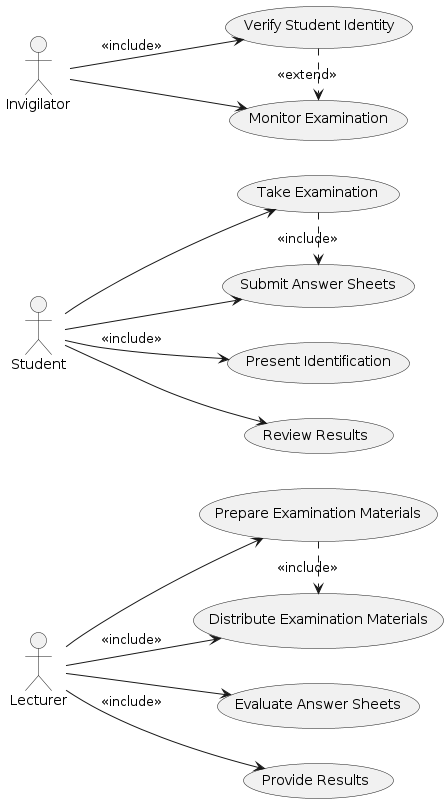
\includegraphics[width=\linewidth]{../figures/usecase_offline_exam}}
	\hfill
	\subcaptionbox{Usecase diagram untuk ujian online.\label{fig:usecase_online_exam}}%
	[0.495\linewidth]{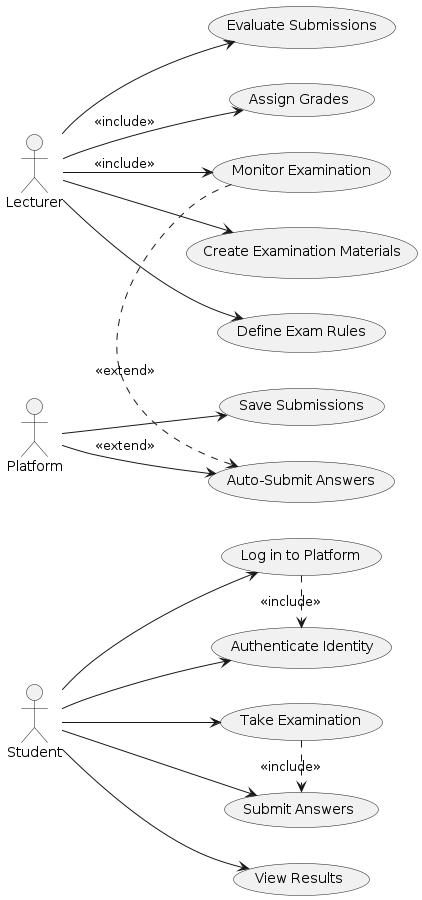
\includegraphics[width=\linewidth]{../figures/usecase_online_exam}}
	\caption{Perbandingan usecase diagram untuk ujian offline dan online.}
\end{figure}

\subsubsection{Sistem Ujian Offline (Baseline)}

Sistem ujian offline mewakili pendekatan tradisional dan manual dalam pelaksanaan ujian. Aktor yang terlibat dalam sistem ini adalah \textbf{Dosen}, \textbf{Mahasiswa}, dan \textbf{Pengawas Ujian}. Interaksi utama antara aktor dan sistem adalah sebagai berikut:

\begin{itemize}
	\item \textbf{Dosen} bertanggung jawab untuk mempersiapkan materi ujian, mendistribusikan materi, mengevaluasi lembar jawaban, dan memberikan hasil. Distribusi materi dan pemberian hasil dimodelkan sebagai hubungan "include", yang menunjukkan bahwa tindakan ini merupakan bagian dari proses yang lebih luas.
	\item \textbf{Mahasiswa} mengikuti ujian, mengumpulkan lembar jawaban, menunjukkan identifikasi untuk verifikasi, dan meninjau hasil ujian. Penyajian identitas dimodelkan sebagai hubungan "include" karena wajib dilakukan untuk mengikuti ujian.
	\item \textbf{Pengawas Ujian} memantau jalannya ujian dan memverifikasi identitas mahasiswa. Proses verifikasi identitas sangat penting dan dimodelkan sebagai hubungan "include". Selain itu, verifikasi identitas memperpanjang proses pemantauan untuk memastikan integritas ujian.
\end{itemize}

Sistem offline, meskipun sudah dikenal, memerlukan intervensi manual di setiap tahap. Alur tugas seperti distribusi, evaluasi, dan verifikasi identitas sangat bergantung pada keterlibatan manusia, yang dapat memakan waktu dan rentan terhadap kesalahan.

\subsubsection{Sistem Ujian Online (Target)}

Sistem ujian online memperkenalkan otomatisasi dan interaksi berbasis platform untuk meningkatkan efisiensi dan skalabilitas. Aktor utama dalam sistem ini adalah \textbf{Dosen}, \textbf{Mahasiswa}, dan \textbf{Platform}. Kegiatan utama dalam sistem ini adalah:

\begin{itemize}
	\item \textbf{Dosen} membuat materi ujian, mendefinisikan aturan ujian, memantau ujian, mengevaluasi kiriman jawaban, dan memberikan nilai. Proses pemantauan mencakup alat otomatis yang disediakan oleh platform untuk meningkatkan efisiensi. Pemberian nilai dimodelkan sebagai hubungan "include" karena merupakan bagian wajib dari evaluasi.
	\item \textbf{Mahasiswa} login ke platform, melakukan autentikasi identitas, mengikuti ujian, mengirim jawaban, dan melihat hasil. Langkah autentikasi sangat penting dalam proses ini, dimodelkan sebagai hubungan "include" untuk memastikan integritas ujian. Pengiriman jawaban juga dimodelkan sebagai tindakan wajib setelah menyelesaikan ujian.
	\item \textbf{Platform} mengotomatiskan beberapa tugas, seperti menyimpan kiriman jawaban dan secara otomatis mengirim jawaban jika mahasiswa tidak melakukannya secara manual sebelum tenggat waktu. Ini dimodelkan sebagai hubungan "extend" untuk menunjukkan bahwa itu terjadi hanya dalam kondisi tertentu (misalnya, waktu habis).
\end{itemize}

Sistem online, dibandingkan dengan yang offline, menawarkan fleksibilitas dan skalabilitas yang lebih besar dengan memungkinkan mahasiswa mengikuti ujian dari jarak jauh dan mengotomatiskan beberapa proses utama, seperti pengiriman dan penilaian. Ini mengurangi beban kerja pada aktor manusia dan memastikan pemantauan ujian yang lebih konsisten melalui kemampuan platform.


\subsection{Activity Diagram}

\begin{figure}[th!]
	\centering
	\subcaptionbox{Activity diagram untuk ujian offline.\label{fig:activity_offline_exam}}%
	[0.49\linewidth]{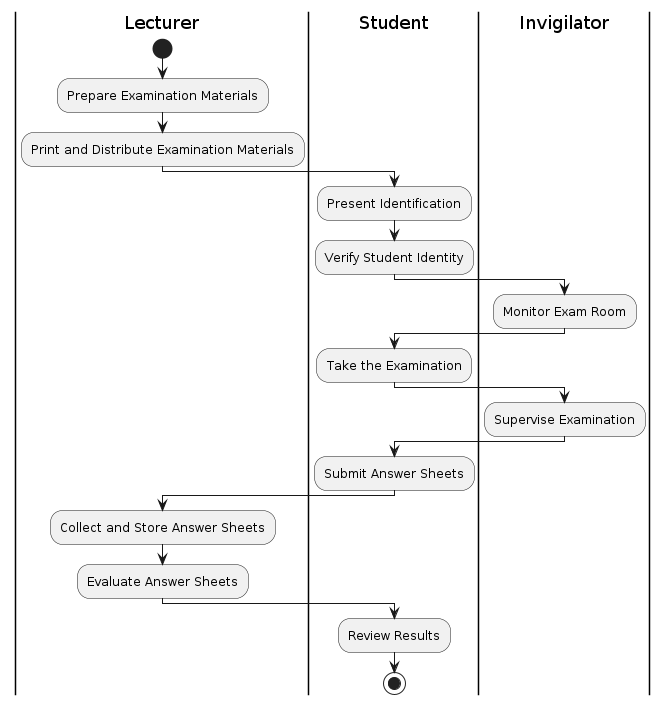
\includegraphics[width=\linewidth]{../figures/activity_offline_exam}}
	\hfill
	\subcaptionbox{Activity diagram untuk ujian online.\label{fig:activity_online_exam}}%
	[0.49\linewidth]{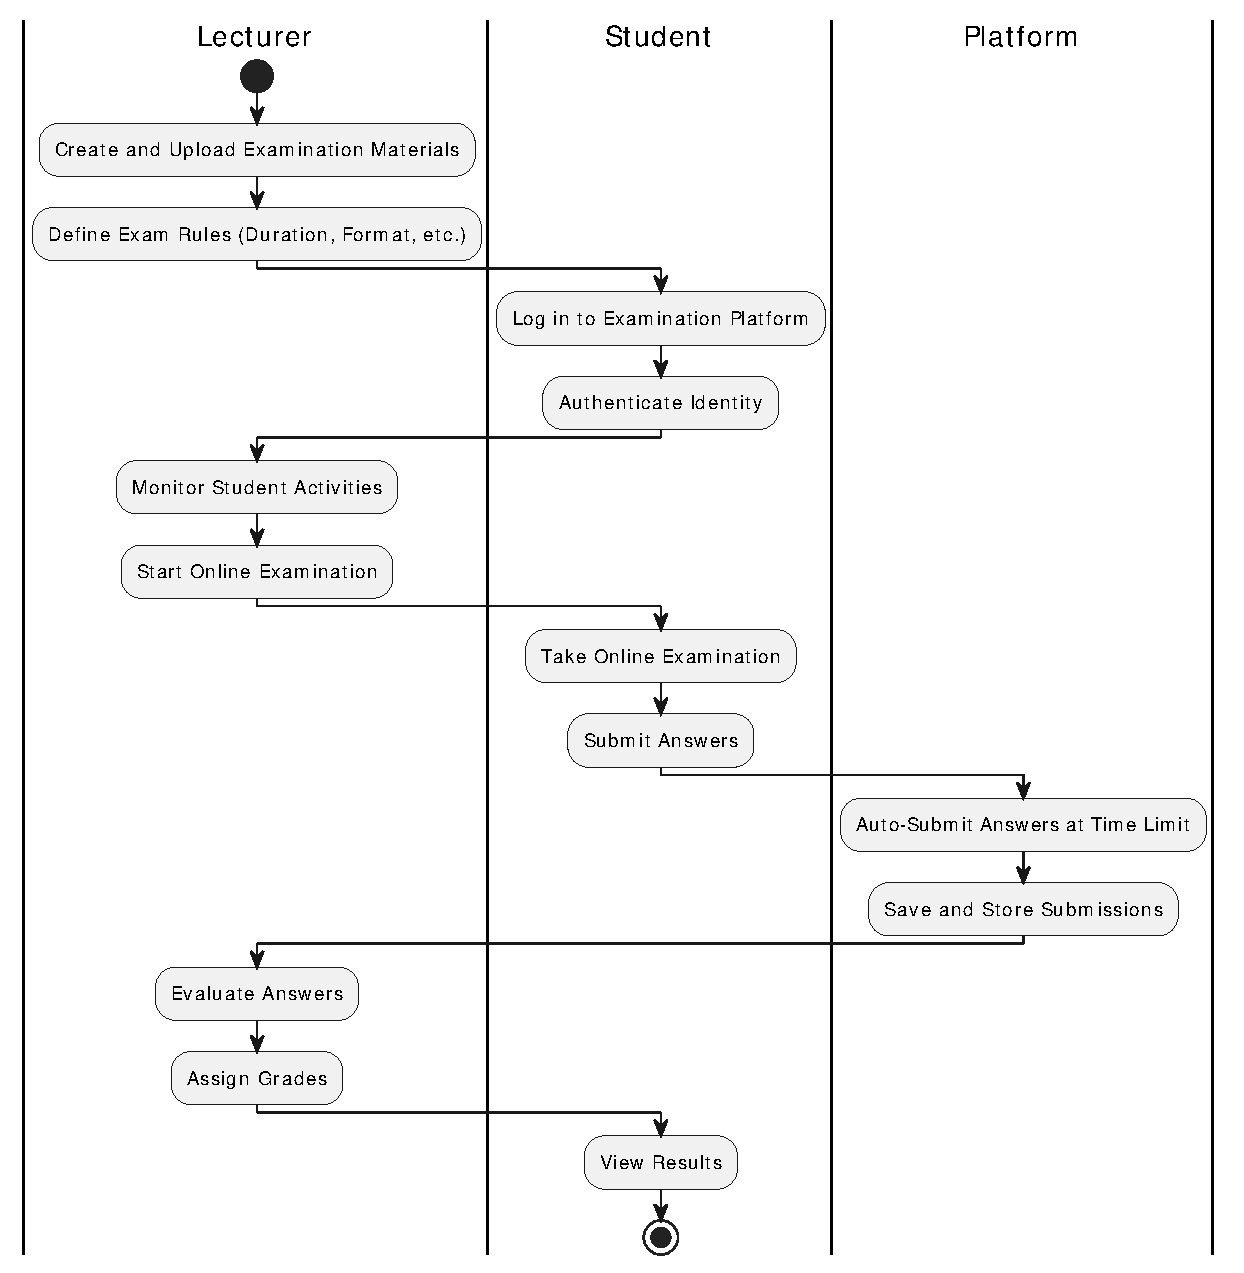
\includegraphics[width=\linewidth]{../figures/activity_online_exam}}
	\caption{Perbandingan activity diagram untuk ujian offline dan online.}
\end{figure}

Activity diagram (Figures \ref{fig:activity_offline_exam} dan \ref{fig:activity_online_exam}) menggambarkan proses ujian pada sistem ujian offline dan online. Setiap diagram menunjukkan alur kerja dari berbagai aktor yang terlibat, seperti dosen, mahasiswa, pengawas, dan platform ujian online.

\subsubsection{Activity Diagram Ujian Offline}

Pada sistem ujian offline, proses ujian dilaksanakan secara manual, mulai dari persiapan hingga evaluasi hasil ujian. Berikut adalah penjelasan dari activity diagram:

\begin{itemize}
	\item \textbf{Dosen} memulai proses dengan mempersiapkan materi ujian, mencetak, dan mendistribusikannya kepada para mahasiswa.
	\item \textbf{Mahasiswa} datang ke ruang ujian dan harus terlebih dahulu menunjukkan identitas diri untuk diverifikasi oleh pengawas. Setelah identitas mahasiswa diverifikasi, mereka dapat mengikuti ujian.
	\item \textbf{Pengawas Ujian} bertanggung jawab untuk memantau ruang ujian selama proses berlangsung, memastikan tidak ada pelanggaran aturan.
	\item Setelah mahasiswa selesai mengerjakan ujian, mereka mengumpulkan lembar jawaban kepada dosen melalui pengawas.
	\item \textbf{Dosen} mengumpulkan, menyimpan, dan kemudian mengevaluasi lembar jawaban tersebut untuk memberikan penilaian.
	\item Setelah proses penilaian selesai, mahasiswa dapat meninjau hasil ujian mereka.
\end{itemize}

Activity diagram ini menunjukkan bahwa setiap tahap dalam proses ujian offline memerlukan interaksi fisik antara mahasiswa, dosen, dan pengawas, serta membutuhkan verifikasi identitas manual dan pengawasan langsung.

\subsubsection{Activity Diagram Ujian Online}

Pada sistem ujian online, banyak aspek dari proses ujian yang diotomatisasi dan difasilitasi oleh platform digital. Berikut adalah penjelasan dari activity diagram:

\begin{itemize}
	\item \textbf{Dosen} memulai dengan membuat dan mengunggah materi ujian ke platform ujian online, serta mendefinisikan aturan ujian, seperti durasi dan format.
	\item \textbf{Mahasiswa} kemudian masuk ke platform ujian online dan melakukan autentikasi identitas sebelum dapat mengikuti ujian.
	\item \textbf{Dosen} memantau aktivitas mahasiswa selama ujian berlangsung dan memulai ujian online sesuai dengan jadwal yang telah ditetapkan.
	\item \textbf{Mahasiswa} mengerjakan ujian di platform, dan jika batas waktu telah tercapai, platform secara otomatis mengirim jawaban yang telah disimpan.
	\item \textbf{Platform} bertanggung jawab untuk menyimpan semua kiriman jawaban yang diunggah oleh mahasiswa, baik secara manual maupun otomatis.
	\item Setelah ujian selesai, \textbf{Dosen} mengevaluasi jawaban dan memberikan penilaian.
	\item \textbf{Mahasiswa} dapat melihat hasil ujian mereka melalui platform setelah penilaian selesai.
\end{itemize}

Activity diagram ini menunjukkan bahwa proses ujian online mengandalkan teknologi untuk mengotomatiskan beberapa tugas penting, seperti autentikasi identitas, pengumpulan jawaban, dan penyimpanan hasil ujian, sehingga mengurangi interaksi fisik dan meningkatkan efisiensi.

\subsection{Archimate Diagram}

\begin{figure}[th!]
	\centering
	\subcaptionbox{Archimate diagram untuk ujian offline.\label{fig:archimate_business_offline_exam}}%
	[0.49\linewidth]{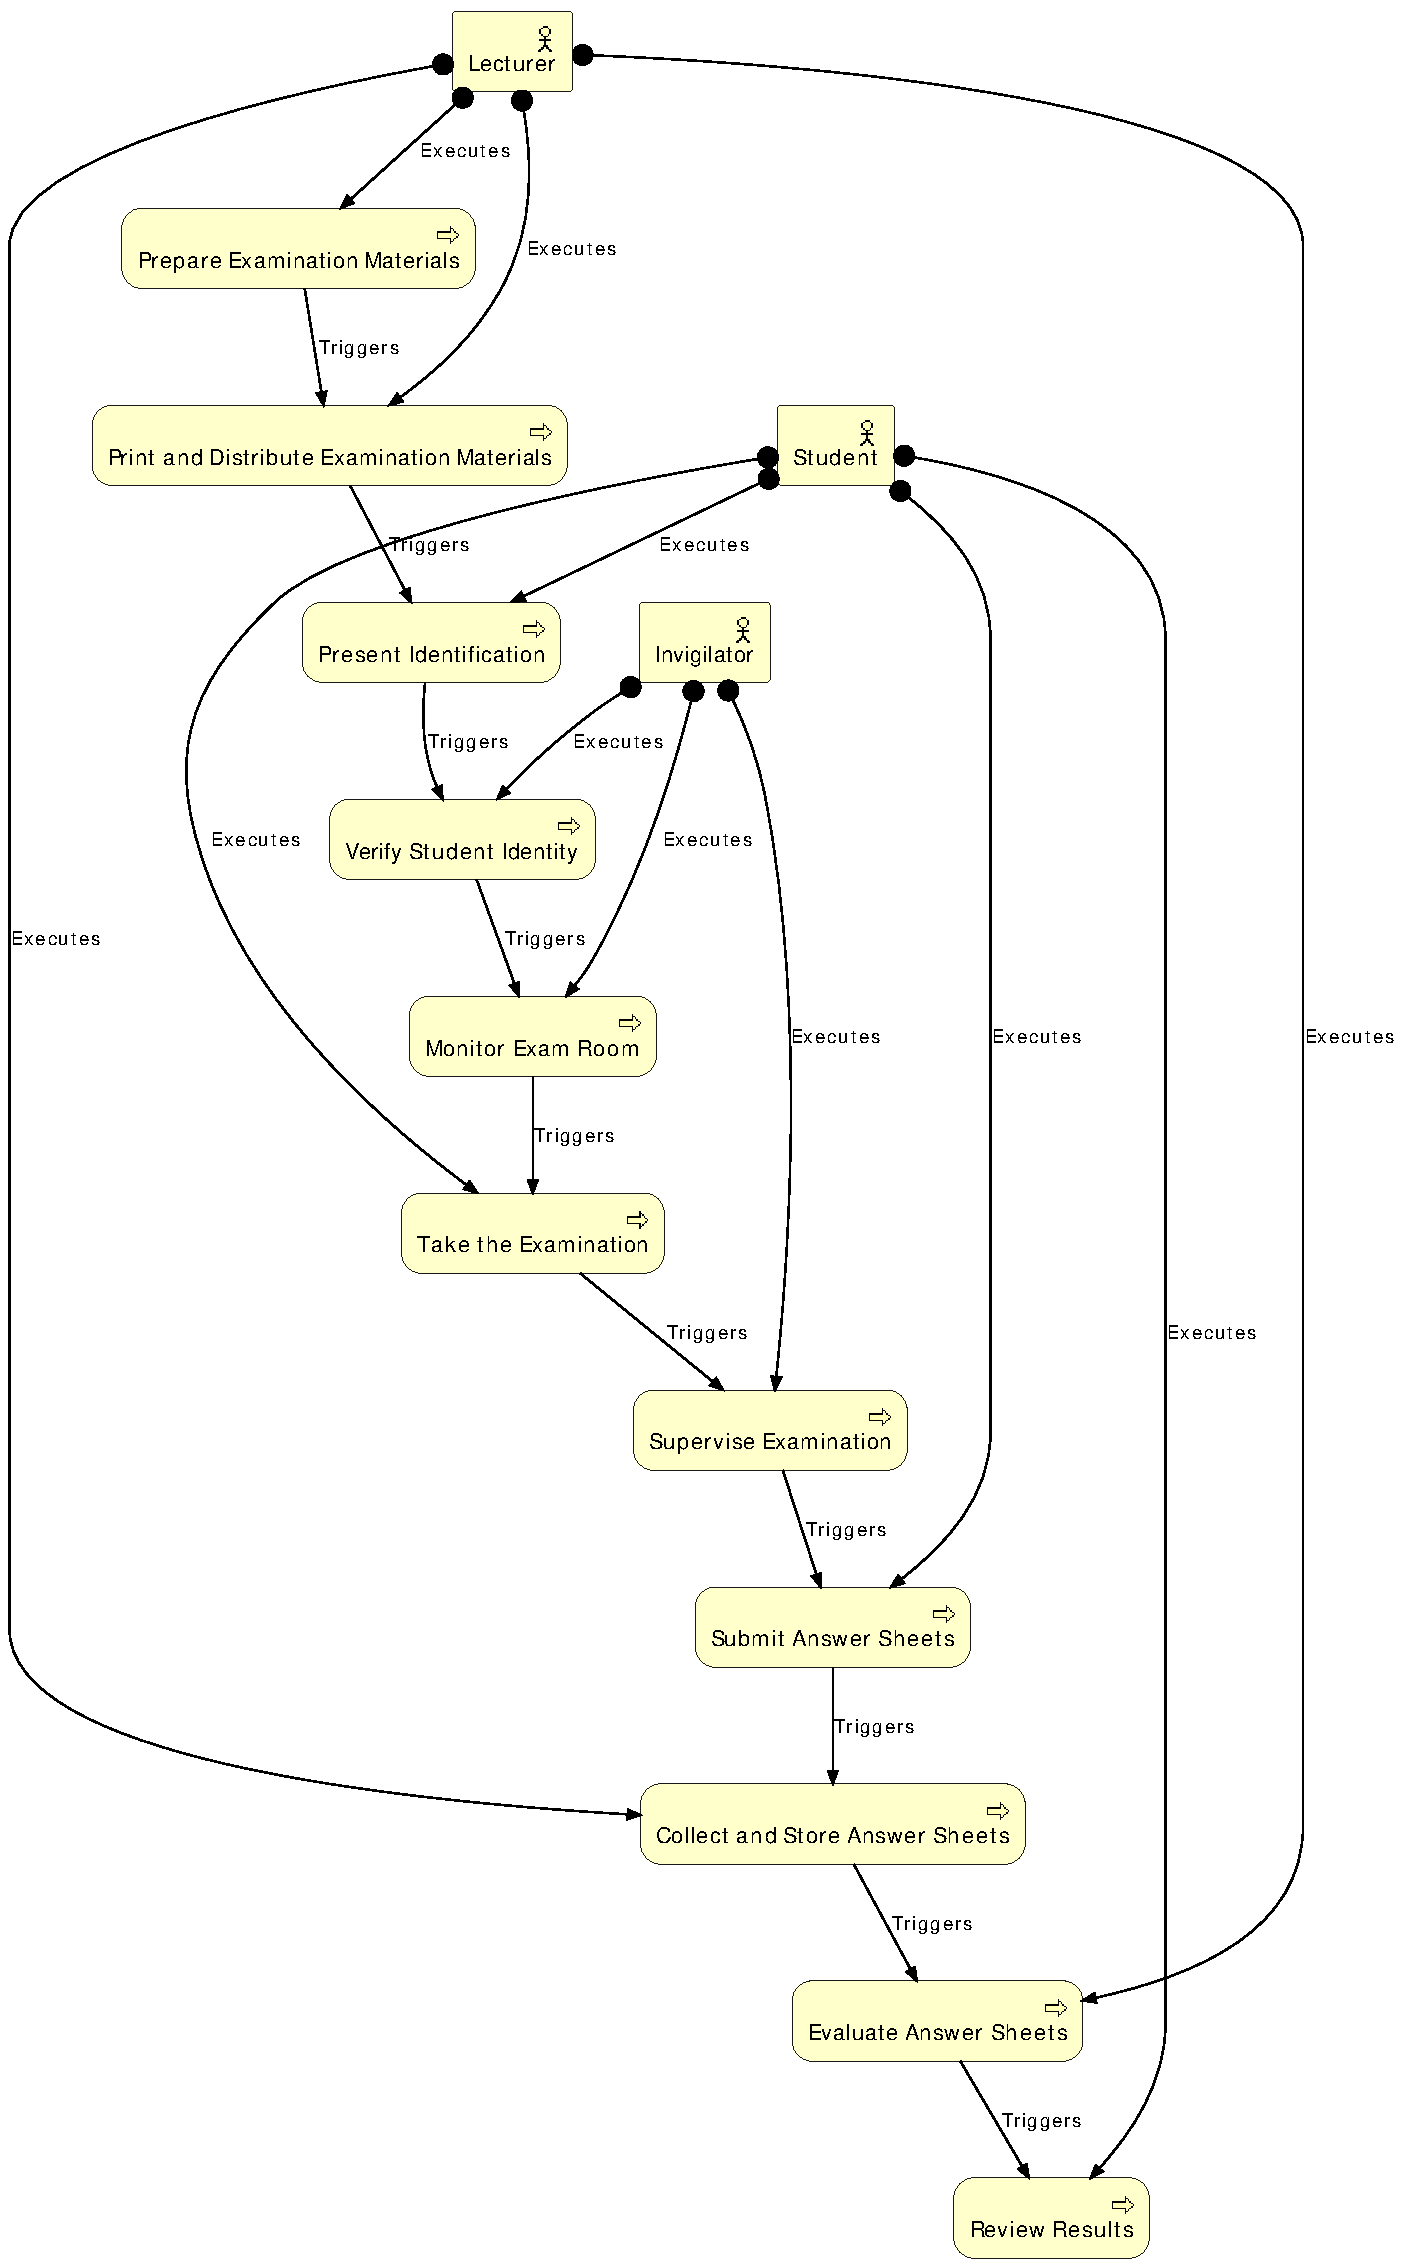
\includegraphics[width=\linewidth]{../figures/archimate_business_offline_exam.pdf}}
	\hfill
	\subcaptionbox{Archimate diagram untuk ujian online.\label{fig:archimate_business_online_exam}}%
	[0.49\linewidth]{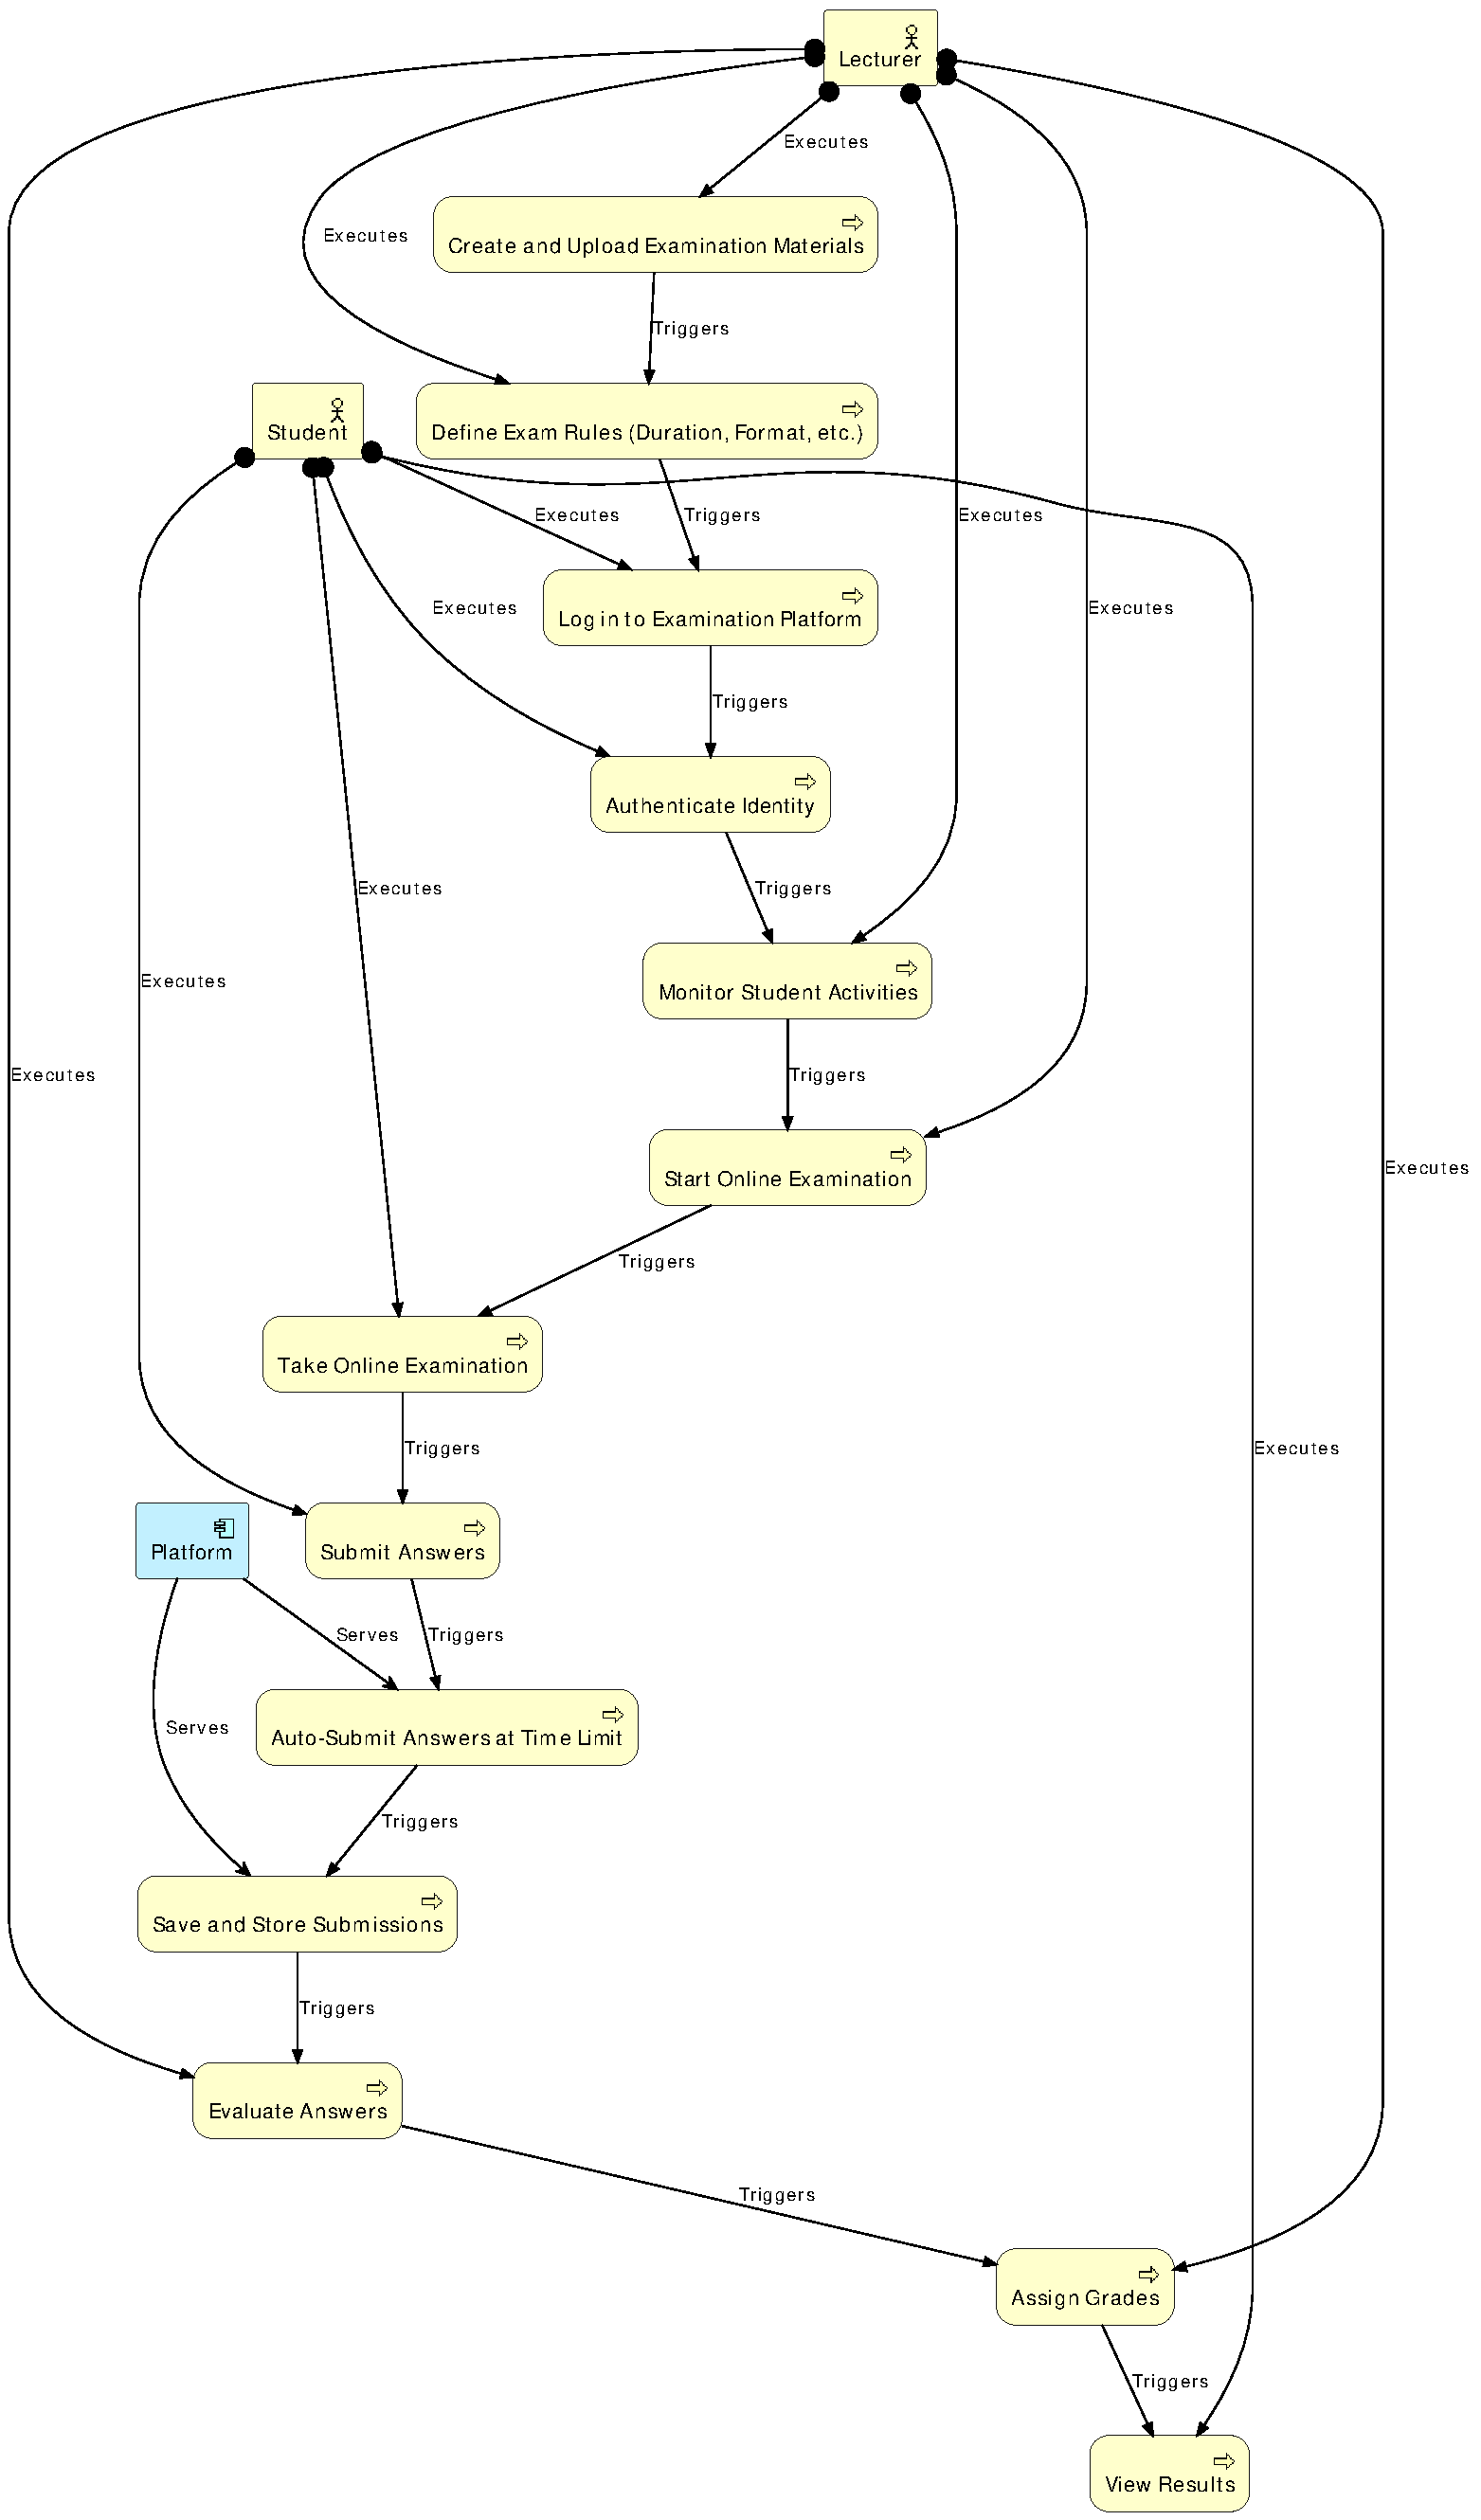
\includegraphics[width=\linewidth]{../figures/archimate_business_online_exam.pdf}}
	\caption{Perbandingan Archimate diagram untuk ujian offline dan online.}
\end{figure}

Pada bagian ini dijelaskan dua ArchiMate diagram yang menggambarkan proses ujian pada sistem ujian offline dan online. Masing-masing diagram menunjukkan alur proses bisnis, aktor yang terlibat, serta hubungan antara proses-proses tersebut.

\subsubsection{ArchiMate Diagram Ujian Offline}

Diagram ArchiMate ujian offline menggambarkan alur proses manual dalam pelaksanaan ujian. Aktor-aktor yang terlibat dalam sistem ini mencakup \textbf{Dosen}, \textbf{Mahasiswa}, dan \textbf{Pengawas Ujian}. Berikut adalah penjelasan detail dari alur proses dalam diagram ini:

\begin{itemize}
	\item \textbf{Dosen} bertanggung jawab untuk mempersiapkan materi ujian, kemudian mencetak dan mendistribusikan materi tersebut kepada mahasiswa.
	\item \textbf{Mahasiswa} harus menunjukkan identifikasi diri sebelum memulai ujian, di mana proses ini diverifikasi oleh pengawas.
	\item \textbf{Pengawas Ujian} bertugas memverifikasi identitas mahasiswa dan memantau ruangan ujian selama ujian berlangsung untuk memastikan kepatuhan terhadap aturan.
	\item Setelah ujian dimulai, \textbf{Mahasiswa} mengerjakan ujian, sementara \textbf{Pengawas} mengawasi jalannya ujian.
	\item Setelah ujian selesai, mahasiswa mengumpulkan lembar jawaban yang kemudian dikumpulkan oleh dosen.
	\item \textbf{Dosen} akan mengevaluasi lembar jawaban dan memberikan hasil kepada mahasiswa untuk ditinjau.
\end{itemize}

Diagram ini menunjukkan alur proses yang ketat dan linear, dengan setiap tahap dalam proses ujian bergantung pada interaksi langsung antara aktor-aktor manusia, serta memerlukan verifikasi manual.

\subsubsection{ArchiMate Diagram Ujian Online}

Diagram ArchiMate ujian online menggambarkan sistem ujian yang difasilitasi oleh platform digital dengan banyak proses yang diotomatisasi. Aktor yang terlibat dalam diagram ini mencakup \textbf{Dosen}, \textbf{Mahasiswa}, dan \textbf{Platform} sebagai komponen aplikasi. Berikut adalah penjelasan prosesnya:

\begin{itemize}
	\item \textbf{Dosen} membuat dan mengunggah materi ujian ke platform, kemudian mendefinisikan aturan ujian seperti durasi dan format ujian.
	\item \textbf{Mahasiswa} masuk ke platform ujian dan mengautentikasi identitas mereka sebelum dapat mengikuti ujian.
	\item Selama ujian berlangsung, \textbf{Dosen} memantau aktivitas mahasiswa melalui platform, dan memulai ujian secara online.
	\item \textbf{Mahasiswa} mengikuti ujian melalui platform, di mana jawaban dapat diserahkan secara manual atau secara otomatis oleh \textbf{Platform} saat batas waktu tercapai.
	\item Platform juga bertanggung jawab untuk menyimpan kiriman jawaban secara otomatis, sementara \textbf{Dosen} mengevaluasi jawaban yang telah disimpan dan memberikan penilaian.
	\item Setelah penilaian selesai, \textbf{Mahasiswa} dapat melihat hasil ujian mereka melalui platform.
\end{itemize}

Diagram ini menekankan peran teknologi dalam mengotomatiskan beberapa proses penting, seperti autentikasi identitas, penyimpanan jawaban, dan pemantauan ujian, yang mengurangi keterlibatan langsung manusia dan meningkatkan efisiensi proses ujian.

Sistem ujian offline memerlukan interaksi langsung antara dosen, mahasiswa, dan pengawas, serta membutuhkan banyak proses manual yang memakan waktu dan rentan terhadap kesalahan. Sebaliknya, sistem ujian online menawarkan otomatisasi yang lebih tinggi dengan platform yang menangani banyak tugas seperti autentikasi, pemantauan, dan penyimpanan jawaban. Hal ini tidak hanya meningkatkan efisiensi tetapi juga memberikan fleksibilitas yang lebih besar bagi dosen dan mahasiswa.


\subsection{Analisis Keuntungan dan Kerugian}

\textbf{Offline (Baseline)}

\textbf{Keuntungan:}
\begin{enumerate}
	\item Proses yang sudah dikenal: Prosedur ujian tradisional yang melibatkan materi fisik dan pengawasan manusia sudah dipahami dengan baik oleh dosen, mahasiswa, dan pengawas.
	\item Pengawasan langsung: Dosen dan pengawas dapat memantau perilaku mahasiswa secara langsung, memungkinkan intervensi segera jika terjadi masalah, seperti kecurangan.
	\item Tidak bergantung pada teknologi: Pendekatan ini tidak mengandalkan platform perangkat lunak, sehingga mengurangi kekhawatiran tentang kegagalan teknis atau keamanan sistem.
\end{enumerate}

\textbf{Kerugian:}
\begin{enumerate}
	\item Memakan waktu: Mempersiapkan, mendistribusikan, dan mengevaluasi materi fisik adalah proses manual yang memerlukan waktu yang cukup lama bagi dosen dan staf administrasi.
	\item Rentan terhadap kesalahan manusia: Proses manual seperti penilaian atau verifikasi identitas mahasiswa dapat menyebabkan ketidakakuratan.
	\item Skalabilitas terbatas: Penanganan ujian untuk jumlah mahasiswa yang besar menjadi tantangan logistik.
	\item Aksesibilitas terbatas: Mahasiswa harus hadir secara fisik untuk mengikuti ujian, yang dapat membatasi fleksibilitas, terutama dalam lingkungan pembelajaran jarak jauh atau hybrid.
\end{enumerate}

\textbf{Online (Target)}

\textbf{Keuntungan:}
\begin{enumerate}
	\item Efisiensi: Proses persiapan dan evaluasi ujian dapat diotomatiskan, dan pengumpulan serta penilaian jawaban dapat dilakukan dengan lebih efisien.
	\item Skalabilitas: Platform digital dapat dengan mudah menangani ujian skala besar, sehingga mengurangi tantangan logistik dari distribusi materi ujian fisik.
	\item Aksesibilitas: Mahasiswa dapat mengikuti ujian dari jarak jauh, yang mendukung model pembelajaran hybrid atau sepenuhnya online.
	\item Manajemen data: Platform secara aman menyimpan kiriman jawaban dan data autentikasi identitas, memberikan proses yang terstruktur dan transparan.
	\item Tindakan otomatis: Fitur seperti pengiriman jawaban otomatis mengurangi risiko mahasiswa kehilangan pekerjaan karena masalah teknis atau batasan waktu.
\end{enumerate}

\textbf{Kerugian:}
\begin{enumerate}
	\item Ketergantungan pada teknologi: Sistem ini sangat bergantung pada ketersediaan dan keandalan platform online, yang dapat mengganggu proses ujian jika terjadi masalah teknis.
	\item Kekhawatiran keamanan: Autentikasi dan pencegahan kecurangan memerlukan langkah-langkah kuat untuk memastikan integritas ujian, yang mungkin memerlukan biaya tambahan.
	\item Kurva belajar: Baik mahasiswa maupun dosen perlu membiasakan diri dengan platform, dan beberapa mungkin menghadapi tantangan dalam beradaptasi dengan teknologi.
\end{enumerate}

\subsection{Analisis Upaya yang Diperlukan untuk Migrasi dari Sistem Ujian Offline (Baseline) ke Online (Target)}

\begin{enumerate}
	
	\item \textbf{Pemilihan dan Penyiapan Platform}
	\begin{enumerate}
		\item Melakukan penelitian dan evaluasi platform ujian online yang memenuhi kebutuhan institusi, dengan fokus pada keamanan, skalabilitas, dan kemudahan penggunaan.
		\item Memperoleh teknologi yang diperlukan, termasuk lisensi platform dan perangkat yang kompatibel dengan sistem.
		\item Mengintegrasikan platform baru dengan sistem informasi mahasiswa (SIS) yang sudah ada untuk mengelola data mahasiswa dan informasi mata kuliah secara efektif.
	\end{enumerate}
	
	\item \textbf{Persiapan dan Konversi Konten}
	\begin{enumerate}
		\item Mengonversi materi ujian yang ada (soal, rubrik penilaian, dll.) ke dalam format digital yang kompatibel dengan platform online.
		\item Mengonfigurasi ujian online di dalam platform, termasuk pengaturan bank soal, aturan ujian, dan kriteria penilaian.
	\end{enumerate}
	
	\item \textbf{Keamanan dan Autentikasi}
	\begin{enumerate}
		\item Mengimplementasikan mekanisme autentikasi yang aman, seperti autentikasi multi-faktor (MFA) atau pengenalan wajah, untuk verifikasi identitas mahasiswa.
		\item Mengintegrasikan alat pengawasan ujian, seperti perangkat lunak proctoring, untuk memantau mahasiswa dan mencegah kecurangan selama ujian.
	\end{enumerate}
	
	\item \textbf{Pelatihan dan Pembiasaan}
	\begin{enumerate}
		\item Memberikan pelatihan kepada dosen tentang cara membuat, memantau, dan menilai ujian menggunakan platform baru.
		\item Menawarkan sesi pelatihan untuk mahasiswa tentang cara login, autentikasi, mengikuti ujian, dan mengirim jawaban di platform.
	\end{enumerate}
	
	\item \textbf{Dukungan Teknis dan Pengujian}
	\begin{enumerate}
		\item Mendirikan tim dukungan teknis khusus untuk membantu mahasiswa dan dosen selama proses ujian.
		\item Melakukan ujian percobaan dengan kelompok kecil mahasiswa dan dosen untuk menguji platform dan mengatasi masalah sebelum implementasi penuh.
	\end{enumerate}
	
	\item \textbf{Komunikasi dan Adaptasi Kebijakan}
	\begin{enumerate}
		\item Menyesuaikan kebijakan ujian yang ada agar sesuai dengan lingkungan online, termasuk aturan tentang verifikasi identitas dan integritas akademik.
		\item Mengkomunikasikan rencana migrasi, kebijakan baru, dan prosedur kepada semua pihak terkait—dosen, mahasiswa, dan staf administrasi—jauh sebelum periode ujian dimulai.
	\end{enumerate}
	
	\item \textbf{Pemantauan dan Iterasi}
	\begin{enumerate}
		\item Secara aktif memantau kinerja platform selama ujian dan memberikan dukungan secara real-time jika diperlukan.
		\item Mengumpulkan umpan balik dari mahasiswa dan dosen setelah ujian untuk meningkatkan proses pada periode ujian berikutnya.
	\end{enumerate}
	
\end{enumerate}

\subsection{Analisis Biaya-Manfaat}

\subsubsection{Biaya}
\begin{enumerate}
	\item Biaya pengaturan awal: Pembelian platform ujian online, termasuk biaya lisensi dan integrasi.
	\item Pelatihan: Waktu dan sumber daya yang digunakan untuk melatih staf dan mahasiswa dalam menggunakan platform baru.
	\item Biaya pemeliharaan: Pengeluaran berkelanjutan untuk memelihara dan mendukung platform, termasuk dukungan teknis.
	\item Manajemen risiko: Investasi tambahan dalam infrastruktur TI atau solusi keamanan untuk mengatasi masalah seperti waktu henti sistem atau pencegahan kecurangan.
\end{enumerate}

\subsubsection{Manfaat}
\begin{enumerate}
	\item Penghematan waktu: Otomatisasi mengurangi beban kerja manual dalam mempersiapkan ujian, menilai jawaban, dan mengelola kiriman.
	\item Skalabilitas: Platform dapat mengakomodasi lebih banyak mahasiswa tanpa meningkatkan beban pada dosen dan staf administrasi.
	\item Aksesibilitas: Mahasiswa dapat mengikuti ujian dari lokasi jarak jauh, meningkatkan fleksibilitas dan mendukung model pembelajaran hybrid.
	\item Manajemen data yang lebih baik: Penyimpanan digital untuk kiriman ujian dan data penilaian memastikan organisasi dan transparansi yang lebih baik.
	\item Umpan balik lebih cepat: Penilaian otomatis memungkinkan mahasiswa menerima umpan balik lebih cepat, yang meningkatkan proses pembelajaran.
\end{enumerate}

Meskipun biaya awal untuk pengaturan sistem ujian online signifikan, manfaat jangka panjang—termasuk penghematan waktu, skalabilitas, dan fleksibilitas—menjadikan transisi ini berharga. Sistem online juga mendukung pembelajaran hybrid, membuatnya menjadi solusi berkelanjutan untuk pendidikan modern.


\section{Aktivitas Kelas dan Tugas}

Buatlah arsitektur bisnis \textbf{As-Is} yang terdampak oleh kapabilitas arsitektur yang dipilih. Juga, buat arsitektur bisnis \textbf{To-Be} yang diperlukan untuk mewujudkan kapabilitas tersebut. 
Expresikan arsitektur bisnis \textbf{As-Is} dan \textbf{To-Be} dalam bentuk Dokumen Definisi Arsitektur (Subbab \ref{sec:isi_dokumen_definisi_arsitektur}) dan Spesifikasi Persyaratan Arsitektur (Subbab \ref{sec:spesifikasi_kebutuhan_arsitektur}).
